\documentclass[10pt,twocolumn,letterpaper]{article}

\usepackage{cvpr}
\usepackage{times}
\usepackage{epsfig}
\usepackage{graphicx}
\usepackage{amsmath}
\usepackage{amssymb}
\usepackage{subfigure}
\usepackage{upgreek}
\usepackage{multirow}
\usepackage{color}
\usepackage{bm}
\DeclareMathOperator*{\argmin}{arg\,min}
\usepackage{arydshln}
\usepackage{cite}


%\usepackage{sectsty}
%\sectionfont{\fontsize{12}{11}\selectfont\leftskip=0pt\vspace{-2mm}}
%\subsectionfont{\fontsize{11}{10}\selectfont\leftskip=0pt\vspace{-1mm}}
%\subsubsectionfont{\fontsize{10}{10}\selectfont\leftskip=0pt\vspace{-1mm}}


% Include other packages here, before hyperref.

% If you comment hyperref and then uncomment it, you should delete
% egpaper.aux before re-running latex.  (Or just hit 'q' on the first latex
% run, let it finish, and you should be clear).
\usepackage[pagebackref=true,breaklinks=true,letterpaper=true,colorlinks,bookmarks=false]{hyperref}

% \cvprfinalcopy % *** Uncomment this line for the final submission

\def\cvprPaperID{1047} % *** Enter the CVPR Paper ID here
\def\httilde{\mbox{\tt\raisebox{-.5ex}{\symbol{126}}}}

% Pages are numbered in submission mode, and unnumbered in camera-ready
\ifcvprfinal\pagestyle{empty}\fi


\begin{document}

%%%%%%%%% TITLE
\title{External Prior Guided Internal Prior Learning for Real Noisy Image Denoising}

\author{First Author\\
Institution1\\
Institution1 address\\
{\tt\small firstauthor@i1.org}
% For a paper whose authors are all at the same institution,
% omit the following lines up until the closing ``}''.
% Additional authors and addresses can be added with ``\and'',
% just like the second author.
% To save space, use either the email address or home page, not both
\and
Second Author\\
Institution2\\
First line of institution2 address\\
{\tt\small secondauthor@i2.org}
}

\maketitle 


%%%%%%%%% ABSTRACT
\begin{abstract}
Most of existing image denoising methods use some statistical models such as additive white Gaussian noise (AWGN) to model the noise, and learn image priors from either external data or the noisy image itself to remove noise.\ However, the noise in real-world noisy images is much more complex than AWGN, and it is hard to be modeled by simple analytical distributions.\ Therefore, many state-of-the-art denoising methods in literature become much less effective when applied to real noisy images.\ In this paper, we develop a robust denoiser for real noisy image denoising without explicit assumption on noise models.\ Specifically, we first learn external priors from a set of clean natural images, and then use the learned external priors to guide the learning of internal priors from the given noisy image for latent clean image recovery.\ The proposed method is simple yet highly effective.\ Experiments on real noisy images demonstrate that it achieves much better denoising performance than state-of-the-art denoising methods, including those designed for real noisy images.
\end{abstract}

%%%%%%%%% BODY TEXT
\section{Introduction} 

Image denoising is a crucial and indispensable step to improve image quality in digital imaging systems.\ In particular, with the decrease of size of CMOS/CCD sensors, image is more easily to be corrupted by noise and hence denoising is becoming increasingly important for high resolution imaging.\ In literature of image denoising, the observed noisy image is usually modeled as $\mathbf{y}=\mathbf{x}+\mathbf{n}$, where $\mathbf{x}$ is the latent clean image and $\mathbf{n}$ is the corrupted noise.\ Numerous image denoising methods \cite{ksvd,lssc,ncsr,nlm,bm3d,cbm3d,pgpd,wnnm,mlp,csf,chen2015learning,foe,epll} have been proposed in the past decades, including sparse representation and dictionary learning based methods \cite{ksvd,lssc,ncsr}, nonlocal self-similarity based methods \cite{ncsr,nlm,bm3d,cbm3d,pgpd}, low-rank based methods \cite{wnnm}, neural network based methods \cite{mlp}, and discriminative learning based methods \cite{csf,chen2015learning}. 

Most of the denoising methods \cite{ksvd,lssc,ncsr,nlm,bm3d,cbm3d,pgpd,wnnm,mlp,csf,chen2015learning,foe,epll} mentioned above assume noise $\mathbf{n}$ to be additive white Gaussian noise (AWGN). Unfortunately, this assumption is too ideal to be true for real-world noisy images, where the noise is much more complex than AWGN \cite{crosschannel2016,healey1994radiometric} and varies by different cameras and camera settings (ISO, shutter speed, and aperture, etc.).\ According to \cite{healey1994radiometric}, the noise corrupted in the imaging process is signal dependent and comes from five main sources:\ photon shot, fixed pattern, dark current, readout, and quantization noise. As a result, many advanced denoising methods in literature becomes much less effective when applied to real-world noisy images.\ Fig.\ \ref{fig1} shows an example, where we apply some representative and state-of-the-art denoising methods, including CBM3D \cite{cbm3d}, WNNM \cite{wnnm}, MLP \cite{mlp}, CSF \cite{csf} and TNRD \cite{chen2015learning}, to a real noisy image (captured by a Nikon D800 camera with ISO is 3200) provided in \cite{crosschannel2016}. One can see that these methods either remain the noise or over-smooth the image details on this real noisy image. 

There have been a few methods \cite{crosschannel2016,Liu2008,almapg,Zhu_2016_CVPR,noiseclinic,ncwebsite,neatimage} developed for real noisy image denoising. Almost all of these methods follow a two-stage framework: first estimate the parameters of the assumed noise model (usually Gaussian  or mixture of Gaussians (MoG)), and then perform denoising with the estimated noise model. Again, the noise in real noisy images is very complex and hard to be modeled by explicit distributions such as Gaussian and MoG.\ Fig.\ \ref{fig1} also shows the denoising results of two state-of-the-art real noisy image denoising methods, Noise Clinic \cite{noiseclinic,ncwebsite} and Neat Image \cite{neatimage}.\ One can see that these two methods do not perform well on this noisy image either. 

\begin{figure*}
\centering
\subfigure{
\begin{minipage}[t]{0.195\textwidth}
\centering
\raisebox{-0.15cm}{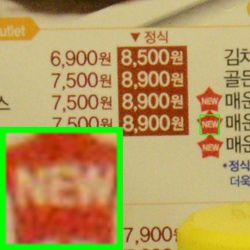
\includegraphics[width=1\textwidth]{images/resize_br_Noisy_CC_Noisy_Nikon_D800_ISO_3200_A3_66.png}}
{\footnotesize (a) Noisy \cite{crosschannel2016}: 33.30dB }
\end{minipage}
\begin{minipage}[t]{0.195\textwidth}
\centering
\raisebox{-0.15cm}{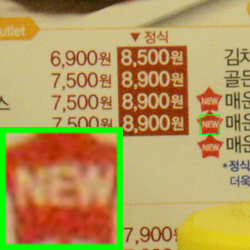
\includegraphics[width=1\textwidth]{images/resize_br_CBM3D_CC_Noisy_Nikon_D800_ISO_3200_A3_66.png}}
{\footnotesize (b) CBM3D \cite{bm3d,cbm3d}: 33.33dB  }
\end{minipage}
\begin{minipage}[t]{0.195\textwidth}
\centering
\raisebox{-0.15cm}{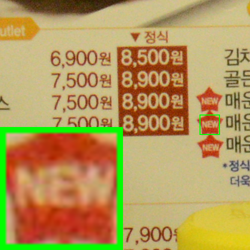
\includegraphics[width=1\textwidth]{images/resize_br_WNNM_CC_Noisy_Nikon_D800_ISO_3200_A3_66.png}}
{\footnotesize (c) WNNM \cite{wnnm}: 33.30dB  }
\end{minipage}
\begin{minipage}[t]{0.195\textwidth}
\centering
\raisebox{-0.15cm}{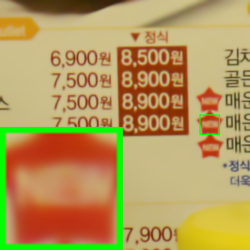
\includegraphics[width=1\textwidth]{images/resize_br_MLP_CC_Noisy_Nikon_D800_ISO_3200_A3_66.png}}
{\footnotesize (d) MLP \cite{mlp}: 34.22dB }
\end{minipage}
\begin{minipage}[t]{0.195\textwidth}
\centering
\raisebox{-0.15cm}{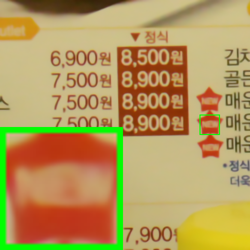
\includegraphics[width=1\textwidth]{images/resize_br_CSF_CC_Noisy_Nikon_D800_ISO_3200_A3_66.png}}
{\footnotesize (e) CSF \cite{csf}: 35.39dB }
\end{minipage}
}\vspace{-3mm}
\subfigure{
\begin{minipage}[t]{0.195\textwidth}
\centering
\raisebox{-0.15cm}{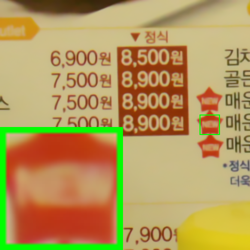
\includegraphics[width=1\textwidth]{images/resize_br_TRD_CC_Noisy_Nikon_D800_ISO_3200_A3_66.png}}
{\footnotesize (f) TNRD \cite{chen2015learning}: 35.97dB   }
\end{minipage}
\begin{minipage}[t]{0.195\textwidth}
\centering
\raisebox{-0.15cm}{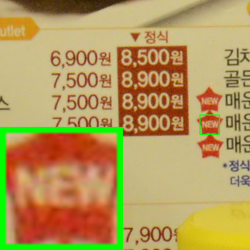
\includegraphics[width=1\textwidth]{images/resize_br_NI_CC_Noisy_Nikon_D800_ISO_3200_A3_66.png}}
{\footnotesize (g) NI \cite{neatimage}: 34.39dB  }
\end{minipage}
\begin{minipage}[t]{0.195\textwidth}
\centering
\raisebox{-0.15cm}{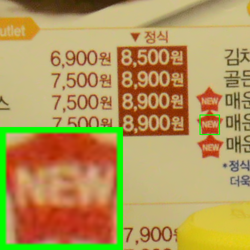
\includegraphics[width=1\textwidth]{images/resize_br_NC_CC_Noisy_Nikon_D800_ISO_3200_A3_66.png}}
{\footnotesize (h) NC \cite{noiseclinic,ncwebsite}: 35.33dB   }
\end{minipage}
\begin{minipage}[t]{0.195\textwidth}
\centering
\raisebox{-0.15cm}{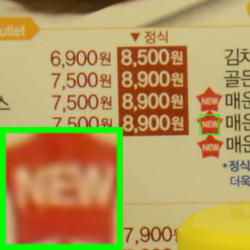
\includegraphics[width=1\textwidth]{images/resize_br_Guided_CC_Noisy_Nikon_D800_ISO_3200_A3_66.png}}
{\footnotesize (i) Ours: \textbf{37.02}dB  }
\end{minipage}
\begin{minipage}[t]{0.195\textwidth}
\centering
\raisebox{-0.15cm}{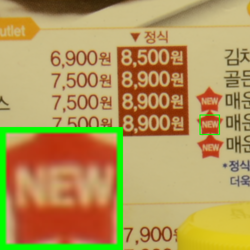
\includegraphics[width=1\textwidth]{images/resize_br_Mean_CC_Noisy_Nikon_D800_ISO_3200_A3_66.png}}
{\footnotesize (j) Mean Image \cite{crosschannel2016} }
\end{minipage}
}\vspace{-1mm}
\caption{Denoised images of a region cropped from the real noisy image ``Nikon D800 ISO 3200 A3" \cite{crosschannel2016} by different methods.\ The scene was shot 500 times with the same camera and camera setting.\ The mean image of the 500 shots is roughly taken as the ``ground truth", with which the PSNR index can be computed. The images are better viewed by zooming in on screen.} 
%\vspace{-1mm}
\label{fig1}
\end{figure*}

This work aims to develop a robust denoiser for real noisy image denoising without explicitly assuming certain noise models.\ To achieve this goal, we propose to first learn image priors from external clean images, and then employ the learned external priors to guide the learning of internal priors from the given noisy image.\ The flowchart of the proposed method is illustrated in\ Fig.\ \ref{fig2}.\ We first extract millions of patch groups from a set of high quality natural images, with which a Gaussian Mixture Model (GMM) is learned as the external prior.\ The learned GMM prior model is used to cluster the patch groups extracted from the given noisy image, and then an external-internal hybrid orthogonal dictionary is learned as the final prior for image denoising. Our proposed denoising method is simple and efficient, yet our extensive experiments on real noisy images clearly demonstrate its better denoising performance than the current state-of-the-arts.

\begin{figure*}\vspace{-2mm}
\centering
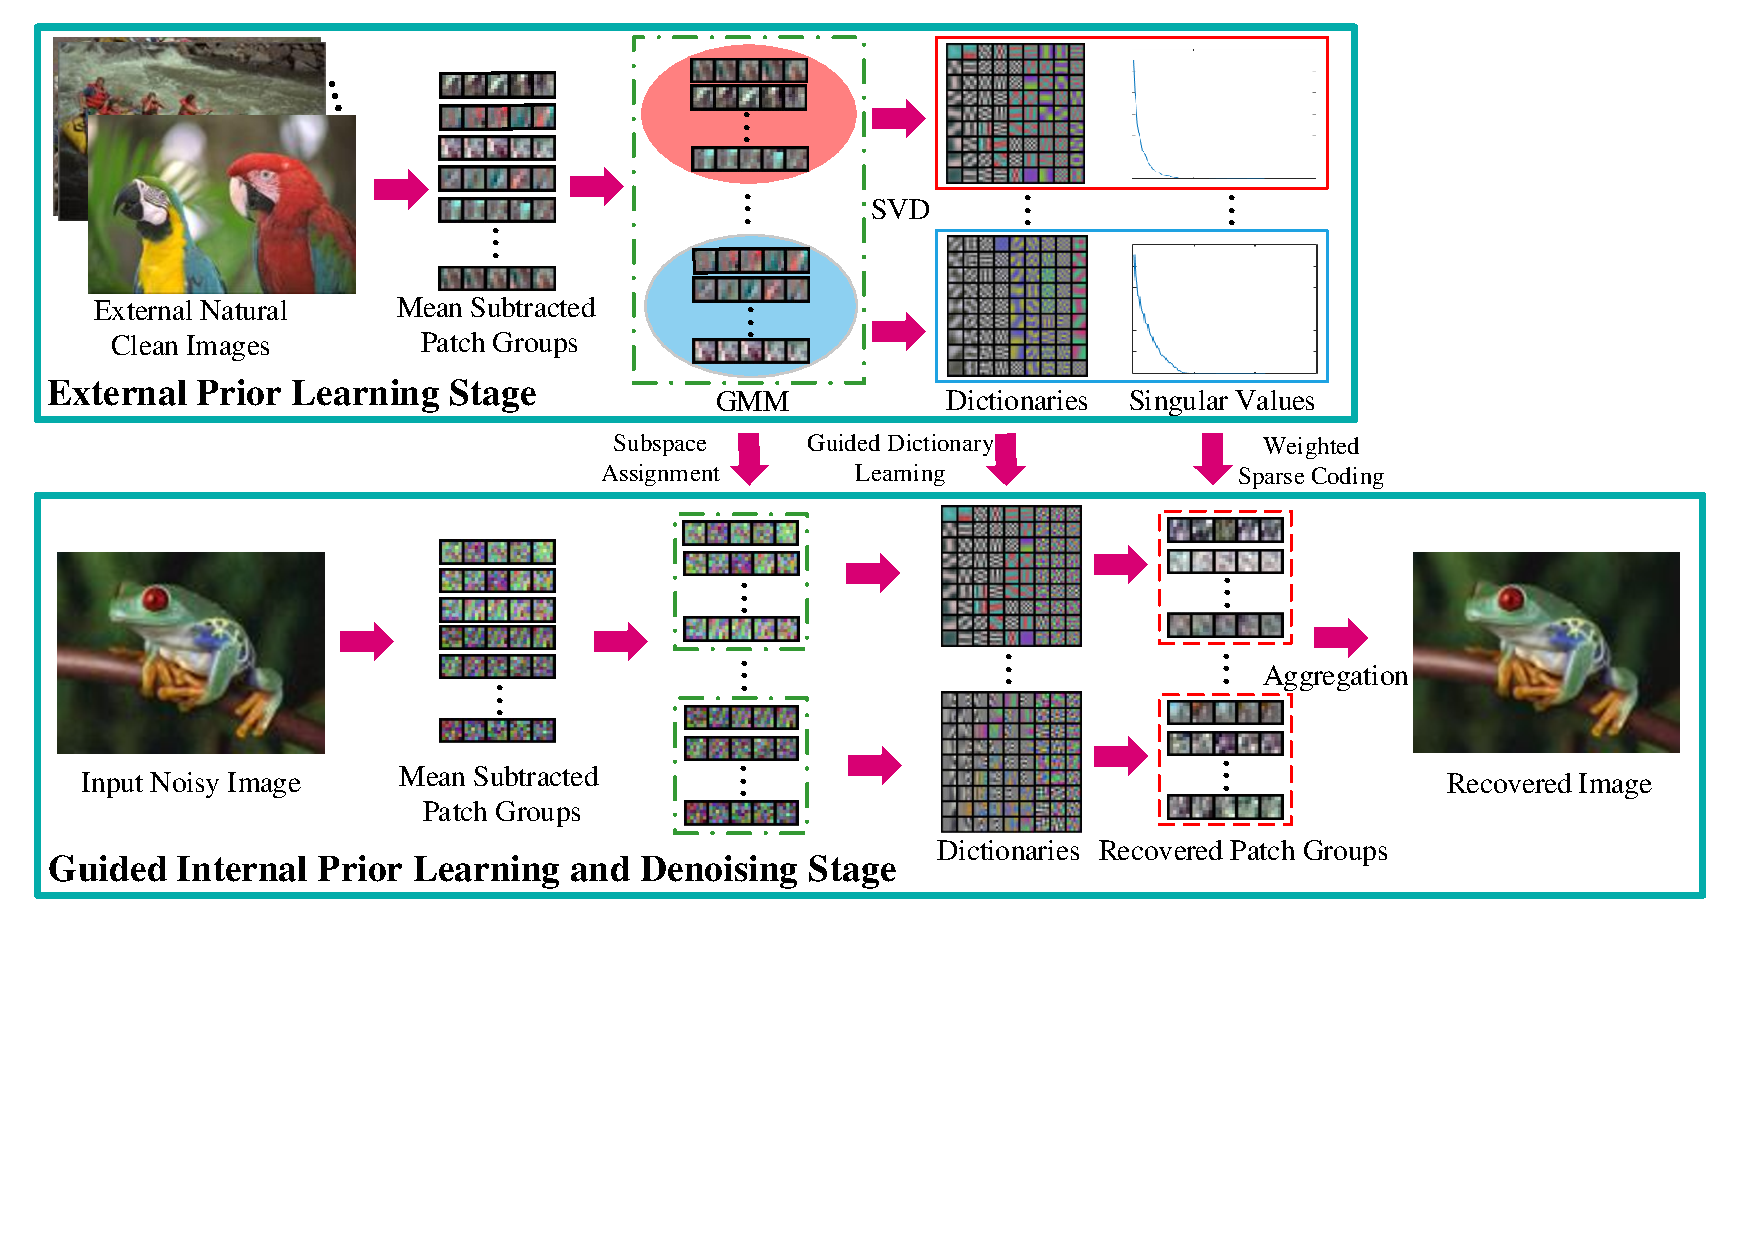
\includegraphics[width=0.95\linewidth]{Flowchart.pdf}
\vspace{-32mm}
\caption{Flowchart of the proposed external prior guided internal prior learning and real noisy image denoising framework.
}
\vspace{-1mm}
\label{fig2}
\end{figure*}

\section{Related Work}

\subsection{Internal \textbf{\emph{vs.}} External Prior Learning}

Image priors are playing a key role in image denoising \cite{ksvd,ncsr,pgpd,foe,epll,ple,iraniinternal}.\ There are mainly two categories of prior learning methods.\ 1) External prior learning methods \cite{pgpd,foe,epll} learn priors (e.g., dictionaries) from a set of external clean images, and the learned priors are used to recover the latent clean image from the given noisy image.\ 2) Internal prior learning methods \cite{ksvd,ncsr,ple,iraniinternal} directly learn priors from the given noisy image, and image denoising is often done simultaneously with the prior learning process.\ It has been demonstrated \cite{pgpd,foe,epll} that the external priors learned from natural clean images are effective and efficient for image denoising problem, but they are not adaptive to the given noisy image so that some fine-scale image structures may not be well recovered.\ By contrast, the internal priors are adaptive to content of the given image, but the learning processing are usually slow.\ In addition, most of the internal prior learning methods \cite{ksvd,ncsr,ple,iraniinternal} assume AWGN noise, making the learned priors less robust for real noisy images. In this paper, we use external priors to guide the internal prior learning.\ Our method is not only much faster than the traditional internal learning methods, but also very effective to denoise real noisy images.

\subsection{Real Noisy Image Denoising}

Recently, several denoising methods have been proposed to remove unknown noise from images \cite{Liu2008,almapg,Zhu_2016_CVPR,noiseclinic,ncwebsite}.\ Among them, the ``Noise Clinic" \cite{noiseclinic,ncwebsite} estimates the noise distribution by using a multivariate Gaussian model and removes the noise by using a generalized version of nonlocal Bayesian model \cite{nlbayes}. Zhu \etal proposed a Bayesian method \cite{Zhu_2016_CVPR} to approximate and remove the noise via a low-rank mixture of Gaussians (MoG) model.\ There are also several methods specifically designed for real noisy image denoising \cite{crosschannel2016,neatimage}.\ The method in \cite{crosschannel2016} models the cross-channel noise in real noisy image as a multivariate Gaussian and the noise is removed by the Bayesian nonlocal means filter \cite{kervrann2007bayesian}.\ The commercial software Neat Image \cite{neatimage} estimates the noise parameters from a flat region of the given noisy image and filters the noise correspondingly.\ Almost all the methods \cite{crosschannel2016,Liu2008,almapg,Zhu_2016_CVPR,noiseclinic,ncwebsite} mentioned above use Gaussian or MoG to model the noise in real noisy images.\ Nonetheless, the noise in real noisy images is very complex and hard to be modeled by explicit distributions.\ In this paper, we propose a simple yet effective method for real noisy image denoising without explicitly assuming certain noise models.

\section{External Prior Guided Internal Prior Learning and Image Denoising}

In this section, we first describe the learning of external prior, and then describe in detail the guided internal prior learning. Finally, the denoising algorithm with the learned priors is presented.

\subsection{Learn External Patch Group Priors}

The nonlocal self-similarity based patch group (PG) \cite{pgpd} has proved to be a very effective unit for image prior learning.\ In this work, we extract PGs from natural clean images to learn priors. A PG is a group of similar patches to a local patch.\ In our method, each local patch is extracted from a RGB image with patch size $p\times p \times 3$.\ We search the $M$ most similar patches to this local patch (including the local patch itself) in a $W\times W$ local region around it. Each patch is stretched to a patch vector $\mathbf{x}_{m}\in \mathbb{R}^{3p^{2}\times1}$ to form the PG $\{\mathbf{x}_{m}\}_{m=1}^{M}$. The mean vector of this PG is $\bm{\mu}=\frac{1}{M}\sum_{m=1}^{M}\mathbf{x}_{m}$, and the group mean subtracted PG is defined as $\mathbf{\overline{X}}\triangleq \{\mathbf{\overline{x}}_{m}=\mathbf{x}_{m}-\bm{\mu}\}_{m=1}^{M}$.

Assume that we have extracted a number of $N$ PGs from a set of external natural images, and the $n$-th PG is $\mathbf{\overline{X}}_{n}\triangleq \{\mathbf{\overline{x}}_{n,m}\}_{m=1}^{M}, n=1,...,N$.\ A Gaussian Mixture Model (GMM) is learned to model the PG prior.\ The overall log-likelihood function is
\vspace{-3mm}
\begin{equation}\label{equ1}\vspace{-2mm}
\begin{split}
\ln\mathcal{L}=\sum_{n=1}^{N} \ln(\sum_{k=1}^{K}\pi_{k}\prod_{m=1}^{M}\mathcal{N}(\mathbf{\overline{x}}_{n,m}|\bm{\mu}_{k},\mathbf{\Sigma}_{k})).
\end{split}
\end{equation}
The learning process is similar to the GMM learning in \cite{pgpd,epll}.\ Finally, a GMM model with $K$ Gaussian components is learned, and the learned parameters include mixture weights $\{\pi_{k}\}_{k=1}^{K}$, mean vectors $\{\bm{\mu}_{k}\}_{k=1}^{K}$, and covariance matrices $\{\mathbf{\Sigma}_{k}\}_{k=1}^{K}$.\ Note that the mean vector of each cluster is naturally zero, i.e., $\bm{\mu}_{k}=\mathbf{0}$.  

To better describe the subspace of each Gaussian component, we perform singular value decomposition (SVD) on the covariance matrix:
\vspace{-2mm}
\begin{equation}\label{equ2}\vspace{-2mm}
\mathbf{\Sigma}_{k}=\mathbf{U}_{k}\mathbf{S}_{k}\mathbf{U}_{k}^{\top}.
\end{equation}
The eigenvector matrices $\{\mathbf{U}_{k}\}_{k=1}^{K}$ will be employed as the external orthogonal dictionary to guide the internal sub-dictionary learning in next sub-section.\ The singular values in $\mathbf{S}_{k}$ reflect the significance of the singular vectors in $\mathbf{U}_{k}$.\ They  will also be utilized as prior weights for weighted sparse coding in our denoising algorithm.

%In Fig.\ \ref{fig3} (a) and (b), we illustrate an external clean image and one orthogonal dictionary learned via GMM on PGs of the external clean image.

\vspace{2mm}
\subsection{Guided Internal Prior Learning}

After the external PG prior is learned on external natural clean images, we employ it to guide the internal PG prior learning for a given real noisy image.\ The guidance lies in two aspects.\ First, the external prior will guide the subspace assignments of internal noisy PGs.\ Second, the external prior will guide the orthogonal dictionary learning of internal noisy PGs.

\vspace{-2mm}
\subsubsection{Internal Subspace Assignment}

Given a real noisy image $\mathbf{y}$, we extract $N$ (overlapped) local patches from it.\ Similar to the external prior learning stage, for the $n$-th local patch we search its $M$ most similar patches around it to form a noisy PG, denoted by $\mathbf{Y}_{n} = \{\mathbf{y}_{n,1},...,\mathbf{y}_{n,M}\}$.\ Then the group mean of $\mathbf{Y}_{n}$, denoted by $\bm{\mu}_{n}$, is subtracted from each patch by $\mathbf{\overline{y}}_{n,m}\triangleq\mathbf{y}_{n,m}-\bm{\mu}_{n}$, leading to the mean subtracted noisy PG $\mathbf{\overline{Y}}_{n}\triangleq \{\mathbf{\overline{y}}_{n,m}\}_{m=1}^{M}$.

The external GMM prior models $\{\mathcal{N}(\mathbf{0},\mathbf{\Sigma}_{k})\}_{k=1}^{K}$ basically characterize the subspaces of natural high quality PGs.\ Therefore, we project the noisy PG $\mathbf{\overline{Y}}_{n}$ into the subspaces of $\{\mathcal{N}(\mathbf{0},\mathbf{\Sigma}_{k})\}_{k=1}^{K}$ and assign it to the most suitable subspace based on the posterior probability:
\vspace{-3mm}
\begin{equation}\label{equ3}\vspace{-2mm}
P(k|\mathbf{\overline{Y}}_{n})=\frac{\prod_{m=1}^{M}\mathcal{N}(\mathbf{\overline{y}}_{n,m}|\mathbf{0},\mathbf{\Sigma}_{k})}{\sum_{l=1}^{K}\prod_{m=1}^{M}\mathcal{N}(\mathbf{\overline{y}}_{n,m}|\mathbf{0},\mathbf{\Sigma}_{l})}
\end{equation}
for $k=1,...,K$.\ Then $\mathbf{\overline{Y}}_{n}$ is assigned to the subspace with the maximum \emph{a}-posteriori (MAP) probability $\max_{k}P(k|\mathbf{\overline{Y}}_{n})$.

\vspace{-2mm}
\subsubsection{Guided Orthogonal Dictionary Learning}

Assume that we have assigned all the internal noisy PGs $\{\mathbf{\overline{Y}}_{n}\}_{n=1}^{N}$ to their corresponding most suitable subspaces in $\{\mathcal{N}(\mathbf{0},\mathbf{\Sigma}_{k})\}_{k=1}^{K}$. For the $k$-th subspace, the noisy PGs assigned to it are $\{\mathbf{\overline{Y}}_{k_{n}}\}_{n=1}^{N_{k}}$ where $\mathbf{\overline{Y}}_{k_{n}}=[\mathbf{\overline{y}}_{k_{n},1},...,\mathbf{\overline{y}}_{k_{n},M}]$ and $\sum_{k=1}^{K}N_{k}=N$.\ We propose to learn an orthogonal dictionary $\mathbf{D}_{k}$ from each set of PGs $\mathbf{\overline{Y}}_{k_{n}}$ to characterize the internal PG prior with the guidance of the corresponding external orthogonal dictionary $\mathbf{U}_{k}$ (Eq.\ (\ref{equ2})). The reasons that we learn orthogonal dictionaries are two-fold.\ Firstly, the PGs $\{\mathbf{\overline{Y}}_{k_{n}}\}_{n=1}^{N_{k}}$ are in a subspace of the whole space of all PGs; therefore, there is no necessary to learn a redundant over-complete dictionary to characterize it, while an orthonormal dictionary has naturally zero \emph{mutual incoherence} \cite{donoho2001uncertainty}. Secondly, the orthogonality of dictionary can make the encoding in the testing stage very efficient, leading to an efficient denoising algorithm (please refer to sub-section 3.3 for more details).

We let the orthogonal dictionary $\mathbf{D}_{k}$ be $\mathbf{D}_{k}\triangleq[\mathbf{D}_{k,\text{E}}\ \mathbf{D}_{k,\text{I}}]\in \mathbb{R}^{3p^2\times 3p^2}$, where $\mathbf{D}_{k,\text{E}}=\mathbf{U}_{k}(:,1:r)\in\mathbb{R}^{3p^2\times r}$ is the external sub-dictionary and it includes the first $r$ most important eigenvectors of $\mathbf{U}_{k}$, and the internal sub-dictionary $\mathbf{D}_{k,\text{I}}$ is to be adaptively learned from the noisy PGs $\{\mathbf{\overline{Y}}_{k_{n}}\}_{n=1}^{N_{k}}$.\ The rationale to design $\mathbf{D}_{k}$ as a hybrid dictionary is as follows.\ The external sub-dictionary $\mathbf{D}_{k,\text{E}}$ is pre-trained from external clean data, and it represents the $k$-th latent subspace of natural images, which is helpful to reconstruct the common latent structures of images. However, $\mathbf{D}_{k,\text{E}}$ is general to all images and it is not adaptive to the given noisy image.\ Some fine-scale details specific to the given image may not be well characterized by $\mathbf{D}_{k,\text{E}}$. Therefore, we learn an internal sub-dictionary $\mathbf{D}_{k,\text{I}}$ to supplement $\mathbf{D}_{k,\text{E}}$.\ In other words, $\mathbf{D}_{k,\text{I}}$ is to reveal the latent subspace adaptive to the input noisy image, which cannot be effectively represented by $\mathbf{D}_{k,\text{E}}$. 

For notation simplicity, in the following development we ignore the subspace index $k$ for $\mathbf{\overline{Y}}_{k_{n}}$ and $\mathbf{D}_{k}$, etc.\ The learning of hybrid orthogonal dictionary $\mathbf{D}$ is performed under the following weighted sparse coding
framework:
\vspace{-2mm}
\begin{equation}\label{equ4}\vspace{-2mm}
\begin{split}
\min_{\mathbf{D}_{\text{I}},\{\bm{\alpha}_{n,m}\}}
&\sum_{n=1}^{N}\sum_{m=1}^{M}(\|\mathbf{\overline{y}}_{n,m}-\mathbf{D}\bm{\alpha}_{n,m}\|_{2}^{2}+\sum_{j=1}^{3p^{2}}\lambda_{j}|\bm{\alpha}_{n,m,j}|)
\\
&
s.t.
\quad
\mathbf{D}=[\mathbf{D}_{\text{E}}\ \mathbf{D}_{\text{I}}],\ \mathbf{D}^{\top}\mathbf{D} = \mathbf{I},
\end{split}
\end{equation}
where $\mathbf{I}$ is the $3p^{2}$ dimensional identity matrix, $\bm{\alpha}_{n,m}$ is the sparse coding vector of the $m$-th patch $\mathbf{\overline{y}}_{n,m}$ in the $n$-th PG $\mathbf{\overline{Y}}_{n}$ and $\bm{\alpha}_{n,m,j}$ is the $j$-th element of $\bm{\alpha}_{n,m}$. $\lambda_{j}$ is the $j$-th regularization parameter defined as
\vspace{-2mm}
\begin{equation}\label{equ5}\vspace{-2mm}
\lambda_{j} = \lambda/(\sqrt{\mathbf{S}_{k}(j)}+\varepsilon),
\end{equation}
where $\mathbf{S}_{k}(j)$ is the $j$-th singular value of diagonal singular value matrix $\mathbf{S}_{k}$ (please refer to Eq.\ (\ref{equ2})) and $\varepsilon$ is a small positive number to avoid zero denominator.\ Note that $\mathbf{D}_{\text{E}}=\mathbf{U}_{k}$ if $r=3p^{2}$ and $\mathbf{D}_{\text{E}}=\emptyset$ if $r=0$.

%The dictionary $\mathbf{D} = [\mathbf{D}_{\text{E}}\ \mathbf{D}_{\text{I}}]$ is orthogonal by checking that:
%\vspace{-2mm}
%\begin{equation}\label{equ6}\vspace{-2mm}
%\mathbf{D}^{\top}\mathbf{D} = 
%\left[\begin{array}{c}
%\mathbf{D}_{\text{E}}^{\top}
%\\
%\mathbf{D}_{\text{I}}^{\top}
%\end{array}\right]
%[\mathbf{D}_{\text{E}}\ \mathbf{D}_{\text{I}}]
%=
%\left[\begin{array}{cc}
%\mathbf{D}_{\text{E}}^{\top}\mathbf{D}_{\text{E}}\ \mathbf{D}_{\text{E}}^{\top}\mathbf{D}_{\text{I}}
%\\
%\mathbf{D}_{\text{I}}^{\top}\mathbf{D}_{\text{E}}\ \mathbf{D}_{\text{I}}^{\top}\mathbf{D}_{\text{I}}
%\end{array}\right]
%=
%\mathbf{I}
%\end{equation}

We employ an alternating iterative approach to solve the optimization problem (\ref{equ4}). Specifically, we initialize the orthogonal dictionary as $\mathbf{D}^{(0)}=\mathbf{U}_{k}$ and for $t=0,1, ...,T-1$, we alternatively update $\bm{\alpha}_{n,m}$ and $\mathbf{D}_{\text{I}}$ as follows.
\vspace{2mm}\\
\textbf{Updating Sparse Coding Coefficients}: Given the orthogonal dictionary $\textbf{D}^{(t)}$, we update each sparse coding vector $\bm{\alpha}_{n,m}$ by solving
\vspace{-4mm}
\begin{equation}\label{equ6}\vspace{-2mm}
\begin{split}
\bm{\alpha}_{n,m}^{(t)}:=\argmin_{\bm{\alpha}_{n,m}}
\|\mathbf{\overline{y}}_{n,m}-\mathbf{D}^{(t)}\bm{\alpha}_{n,m}\|_{2}^{2}+\sum_{j=1}^{3p^{2}}\lambda_{j}|\bm{\alpha}_{n,m,j}|
\end{split}
\end{equation}
Since dictionary $\mathbf{D}^{(t)}$ is orthogonal, the problems (\ref{equ6}) has a closed-form solution
\vspace{-1mm}
\begin{equation}\label{equ7}\vspace{-0mm}
\bm{\alpha}_{n,m}^{(t)}= \text{sgn}((\mathbf{D}^{(t)})^{\top}\mathbf{\overline{y}}_{n,m})\odot \text{max}(|(\mathbf{D}^{(t)})^{\top}\mathbf{\overline{y}}_{n,m}|-\bm{\lambda},\mathbf{0}),
\end{equation}
where $\bm{\lambda} = [\lambda_{1},\lambda_{2},...,\lambda_{3p^2}]$ is the vector of regularization parameter, $\text{sgn}(\bullet)$ is the sign function and $\odot$ means element-wise multiplication.\ The detailed derivation of Eq. (\ref{equ7}) can be found in the supplementary file.
\vspace{2mm}\\
\textbf{Updating Internal Sub-dictionary}: Given the sparse coding vectors $\{\bm{\alpha}_{n,m}^{(t)}\}$, we update the internal sub-dictionary by solving
\vspace{-3mm}
\begin{equation}\label{equ8} \vspace{-2mm}
\begin{split}
\textbf{D}_{\text{I}}^{(t+1)}
:
&
=
\argmin_{\textbf{D}_{\text{I}}}
\sum_{n=1}^{N}\sum_{m=1}^{M}\|\mathbf{\overline{y}}_{n,m}-\mathbf{D}\bm{\alpha}_{n,m}^{(t)}\|_{2}^{2}
\\
&
=
\argmin_{\textbf{D}_{\text{I}}}
\|\mathbf{Y}-\mathbf{D}\mathbf{A}^{(t)}\|_{F}^{2}
\\
s.t.
\quad
\mathbf{D}
&
=
[\mathbf{D}_{\text{E}}\ \mathbf{D}_{\text{I}}],\ \mathbf{D}_{\text{I}}^{\top}\mathbf{D}_{\text{I}} = \mathbf{I}_{(3p^2-r)},\ \mathbf{D}_{\text{E}}^{\top}\mathbf{D}_{\text{I}} = \mathbf{0},
\end{split}
\end{equation}
where $\textbf{A}^{(t)}=[\bm{\alpha}_{1,1}^{(t)},...,\bm{\alpha}_{1,M}^{(t)},...,\bm{\alpha}_{N,1}^{(t)},...,\bm{\alpha}_{N,M}^{(t)}]$ and $\mathbf{I}_{(3p^2-r)}$ is the $(3p^2-r)$ dimensional identity matrix.\ The sparse coefficients matrix can be written as $\mathbf{A}^{(t)}=[(\mathbf{A}_{\text{E}}^{(t)})^{\top}\ (\mathbf{A}_{\text{I}}^{(t)})^{\top}]^{\top}$ where the external part $\mathbf{A}_{\text{E}}^{(t)}\in\mathbb{R}^{r\times NM}$ and the internal part $\mathbf{A}_{\text{I}}^{(t)}\in\mathbb{R}^{(3p^2-r)\times NM}$ represent the coding coefficients of $\mathbf{Y}$ over external sub-dictionary $\mathbf{D}_{\text{E}}$ and internal sub-dictionary $\mathbf{D}_{\text{I}}^{(t)}$, respectively.\ According to the Theorem 4 in \cite{spca}, the problem (\ref{equ8}) has a closed-form solution $\mathbf{D}_{\text{I}}^{(t+1)}=\mathbf{U}_{\text{I}}\mathbf{V}_{\text{I}}^{\top}$, where $\mathbf{U}_{\text{I}}\in\mathbb{R}^{3p^2\times (3p^2-r)}$ and $\mathbf{V}_{\text{I}}\in\mathbb{R}^{(3p^2-r)\times (3p^2-r)}$ are the orthogonal matrices obtained by the following SVD
\vspace{-2mm}
\begin{equation}\label{equ9}\vspace{-2mm}
(\mathbf{I}-\mathbf{D}_{\text{E}}\mathbf{D}_{\text{E}}^{\top})\mathbf{Y}(\mathbf{A}_{\text{I}}^{(t)})^{\top}
=
\mathbf{U}_{\text{I}}\mathbf{S}_{\text{I}}\mathbf{V}_{\text{I}}^{\top}.
\end{equation}
The orthogonality of internal sub-dictionary $\mathbf{D}_{\text{I}}^{(t+1)}$ can be checked by 
$(\mathbf{D}_{\text{I}}^{(t+1)})^{\top}(\mathbf{D}_{\text{I}}^{(t+1)})=\mathbf{V}_{\text{I}}\mathbf{U}_{\text{I}}^{\top}\mathbf{U}_{\text{I}}\mathbf{V}_{\text{I}}^{\top}=\mathbf{I}_{(3p^2-r)}$.
%In Fig. \ref{fig3} (c) and (d), we illustrate a denoised image by our proposed method and one internal orthogonal dictionary learned from PGs of the given noisy image.

\subsection{The Denoising Algorithm}

The denoising of the given noisy image $\mathbf{y}$ can be simultaneously done with the guided internal sub-dictionary learning process. Once we obtain the solutions of sparse coding vectors $\{\hat{\bm{\alpha}}_{n,m}^{(T-1)}\}$ in Eq.\ (\ref{equ7}) and the orthogonal dictionary $\mathbf{D}^{(T)} = [\mathbf{D}_{\text{E}}\ \mathbf{D}_{\text{I}}^{(T)}]$ in Eq.\ (\ref{equ8}), the latent clean patch $\hat{\mathbf{y}}_{n,m}$ of the $m$-th noisy patch in PG $\mathbf{Y}_{n}$ is reconstructed as
\vspace{-2mm}
\begin{equation}\label{equ10}\vspace{-2mm}
\hat{\mathbf{y}}_{n,m}=\mathbf{D}^{(T)}\hat{\bm{\alpha}}_{n,m}^{(T-1)}+\bm{\mu}_{n},
\end{equation}
where $\bm{\mu}_{n}$ is the group mean of $\mathbf{Y}_{n}$. The latent clean image is then reconstructed by aggregating all the reconstructed patches in all PGs.\ We perform the above denoising procedures for several iterations for better denoising outputs.\ The proposed denoising algorithm is summarized in Alg. 1.
\begin{table}\label{alg1}
\begin{tabular}{l}
\hline
\textbf{Alg. 1}: External Prior Guided Internal Prior Learning
\\
\quad \quad \quad for Real Noisy Image Denoising
\\
\hline
\textbf{Input:} Noisy image $\mathbf{y}$, external PG prior GMM model
\\
\textbf{Output:} The denoised image $\hat{\mathbf{x}}$.
\\
\textbf{Initialization:} $\hat{\mathbf{x}}^{(0)}=\mathbf{y}$;
\\
\textbf{for} $Ite = 1:IteNum$ \textbf{do}
\\
1. Extracting internal PGs $\{\mathbf{Y}_{n}\}_{n=1}^{N}$ from $\hat{\mathbf{x}}^{(Ite-1)}$;
\\
%\textbf{Guided Internal Subspace Assignment:}
%\\
\quad\textbf{for} each PG $\mathbf{Y}_{n}$ \textbf{do}
\\
2.\quad Calculate group mean vector $\bm{\mu}_{n}$ and form 
\\
\quad \ \ \ mean subtracted PG $\mathbf{\overline{Y}}_{n}$;
\\
3.\quad Subspace assignment via Eq. (\ref{equ3});
\\
\quad\textbf{end for}
\\
%\textbf{Guided Internal Orthogonal Dictionary Learning:}
%\\
\quad\textbf{for} the PGs in each subspace \textbf{do}
\\
4.\quad External PG prior guided internal orthogonal
\\
\quad \ \ \ dictionary learning by solving (\ref{equ4});
\\
5.\quad Recover each patch in all PGs via Eq. (\ref{equ10});
\\
\quad\textbf{end for}
\\
6. Aggregate the recovered PGs of all subspaces to form
\\
\quad the recovered image $\hat{\mathbf{x}}^{(Ite)}$;
\\
\textbf{end for}
\\
\hline
\end{tabular}
\end{table}


%------------------------------------------------------------------------

\section{Experiments}\vspace{-1mm}

We evaluate the performance of the proposed algorithm on real-world noisy images \cite{crosschannel2016,ncwebsite}  in comparison with  state-of-the-art denoising methods \cite{bm3d,cbm3d,mlp,wnnm,csf,chen2015learning,crosschannel2016,noiseclinic,ncwebsite,neatimage}.


\subsection{Implementation Details}\vspace{-1mm}

Our proposed method has two stages: the external prior learning stage and the external prior guided internal prior learning stage.\ In the first stage, we set $p = 6$ (the patch size), $M = 10$ (the number of similar patches in a PG), $W = 31$ (the window size for PG searching) and $K = 32$ (the number of Gaussian components in GMM).\ We learn the external GMM prior with 3.6 million PGs extracted from the Kodak PhotoCD Dataset (\url{http://r0k.us/graphics/kodak/}), which includes 24 high quality color images. 

In the second stage, we set $r = 54$ (the number of atoms in the external sub-dictionaries); that is, we let the external sub-dictionaries have the same number of atoms as the internal sub-dictionaries to be learned. Our experiments show that setting $r$ between 27 and 81 will lead to very similar results. For other parameters, we set $\lambda=0.001$ (the sparse regularization parameter), $T = 2$ (the number of iterations for solving problem (\ref{equ4})), and $IteNum = 4$ (the number of iterations for Alg.1). All parameters of our method are fixed to all experiments, which are run under the Matlab2014b environment on a machine with Intel(R) Core(TM) i7-5930K CPU of 3.5GHz and 32GB RAM.


\subsection{The Testing Datasets}\vspace{-1mm}

We evaluate the proposed method on two real noisy image datasets, where the images were captured under indoor or outdoor lighting conditions by different types of cameras and camera settings. 

The first dataset is provided in \cite{ncwebsite}, which includes 20 real noisy images collected under uncontrolled outdoor environment.\ Since there is no ``ground truth" of the noisy images, the objective measures such as PSNR cannot be computed on this dataset. 

The second dataset is provided in \cite{crosschannel2016}, which includes noisy images of 17 static scenes.\ The noisy images were collected under controlled indoor environment.\ Each scene was shot 500 times under the same camera and camera setting.\ The mean image of the 500 shots is roughly taken as the ``ground truth", with which the PSNR can be computed. Since the image size is very large (about $7000\times5000$) and the 17 scenes share repetitive contents, the authors of \cite{crosschannel2016} cropped 15 smaller images (of size $512\times512$) to perform experiments.\ To more comprehensively evaluate the proposed methods, we cropped 60 images of size $500\times500$ from the dataset for experiments. Some samples are shown in Fig.\ \ref{fig3}.\ Note that the noise in our cropped 60 images is different from the noise in the 15 images cropped by the authors of \cite{crosschannel2016} since they are from different shots.

\begin{figure}[t]
\centering
\subfigure{
\begin{minipage}{0.055\textwidth}
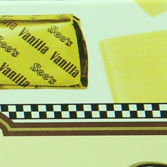
\includegraphics[width=1\textwidth]{images/resize_CC_Noisy_Canon_EOS_5D_Mark3_ISO_3200_C1_47.png}
\end{minipage}
\begin{minipage}{0.055\textwidth}
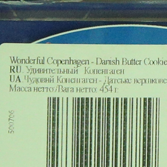
\includegraphics[width=1\textwidth]{images/resize_CC_Noisy_Canon_EOS_5D_Mark3_ISO_3200_C1_52.png}
\end{minipage}
\begin{minipage}{0.055\textwidth}
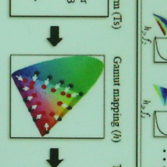
\includegraphics[width=1\textwidth]{images/resize_CC_Noisy_Canon_EOS_5D_Mark3_ISO_3200_C2_44.png}
\end{minipage}
\begin{minipage}{0.055\textwidth}
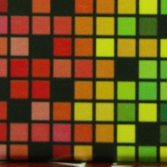
\includegraphics[width=1\textwidth]{images/resize_CC_Noisy_Canon_EOS_5D_Mark3_ISO_3200_C2_66.png}
\end{minipage}
\begin{minipage}{0.055\textwidth}
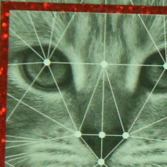
\includegraphics[width=1\textwidth]{images/resize_CC_Noisy_Canon_EOS_5D_Mark3_ISO_3200_C3_26.png}
\end{minipage}
\begin{minipage}{0.055\textwidth}

\includegraphics[width=1\textwidth]{images/resize_CC_Noisy_Canon_EOS_5D_Mark3_ISO_3200_C3_73.png}
\end{minipage}
\begin{minipage}{0.055\textwidth}
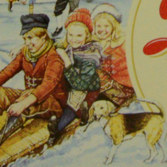
\includegraphics[width=1\textwidth]{images/resize_CC_Noisy_Nikon_D600_ISO_3200_C1_95.png}
\end{minipage}
\begin{minipage}{0.055\textwidth}
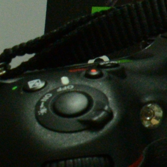
\includegraphics[width=1\textwidth]{images/resize_CC_Noisy_Nikon_D600_ISO_3200_C2_67.png}
\end{minipage}
}\vspace{-3mm}
\subfigure{
\begin{minipage}{0.055\textwidth}
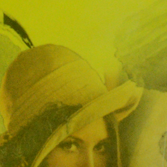
\includegraphics[width=1\textwidth]{images/resize_CC_Noisy_Nikon_D800_ISO_1600_B2_80.png}
\end{minipage}
\begin{minipage}{0.055\textwidth}
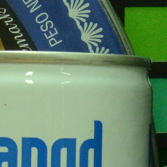
\includegraphics[width=1\textwidth]{images/resize_CC_Noisy_Nikon_D800_ISO_1600_B3_82.png}
\end{minipage}
\begin{minipage}{0.055\textwidth}
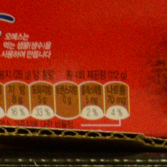
\includegraphics[width=1\textwidth]{images/resize_CC_Noisy_Nikon_D800_ISO_3200_A1_21.png}
\end{minipage}
\begin{minipage}{0.055\textwidth}
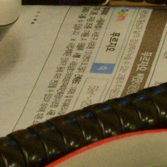
\includegraphics[width=1\textwidth]{images/resize_CC_Noisy_Nikon_D800_ISO_3200_A1_111.png}
\end{minipage}
\begin{minipage}{0.055\textwidth}
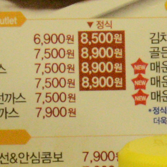
\includegraphics[width=1\textwidth]{images/resize_CC_Noisy_Nikon_D800_ISO_3200_A3_66.png}
\end{minipage}
\begin{minipage}{0.055\textwidth}
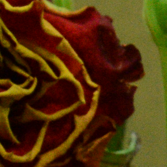
\includegraphics[width=1\textwidth]{images/resize_CC_Noisy_Nikon_D800_ISO_3200_A4_51.png}
\end{minipage}
\begin{minipage}{0.055\textwidth}
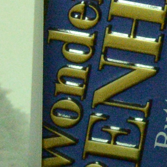
\includegraphics[width=1\textwidth]{images/resize_CC_Noisy_Nikon_D800_ISO_6400_B3_95.png}
\end{minipage}
\begin{minipage}{0.055\textwidth}
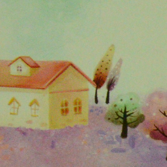
\includegraphics[width=1\textwidth]{images/resize_CC_Noisy_Nikon_D800_ISO_3200_A2_80.png}
\end{minipage}
}
\caption{Some samples cropped from real noisy images of \cite{crosschannel2016}.}
\label{fig3}
\vspace{-2mm}
\end{figure}


\begin{figure*}\vspace{-1mm}
\centering
\subfigure{
\begin{minipage}[t]{0.195\textwidth}
\centering
\raisebox{-0.15cm}{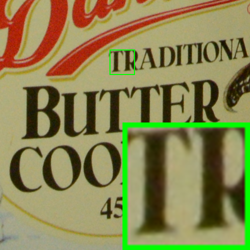
\includegraphics[width=1\textwidth]{images/resize_br_Noisy_CC_Noisy_Nikon_D600_ISO_3200_C1_96.png}}
{\footnotesize (a) Noisy \cite{crosschannel2016}: 35.89dB  }
\end{minipage}
\begin{minipage}[t]{0.195\textwidth}
\centering
\raisebox{-0.15cm}{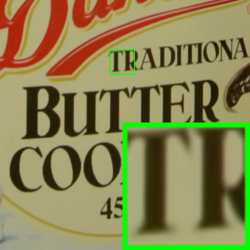
\includegraphics[width=1\textwidth]{images/resize_br_Offline_CC_Noisy_Nikon_D600_ISO_3200_C1_96.png}}
{\footnotesize (b) External: 39.05dB }
\end{minipage}
\begin{minipage}[t]{0.195\textwidth}
\centering
\raisebox{-0.15cm}{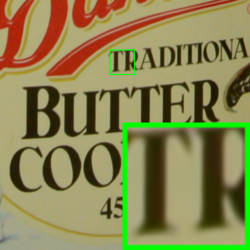
\includegraphics[width=1\textwidth]{images/resize_br_Online_CC_Noisy_Nikon_D600_ISO_3200_C1_96.png}}
{\footnotesize (c) Internal: 38.75dB }
\end{minipage}
\begin{minipage}[t]{0.195\textwidth}
\centering
\raisebox{-0.15cm}{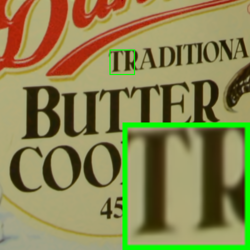
\includegraphics[width=1\textwidth]{images/resize_br_Guided_CC_Noisy_Nikon_D600_ISO_3200_C1_96.png}}
{\footnotesize (d) Guided Internal: \textbf{39.39}dB }
\end{minipage}
\begin{minipage}[t]{0.195\textwidth}
\centering
\raisebox{-0.15cm}{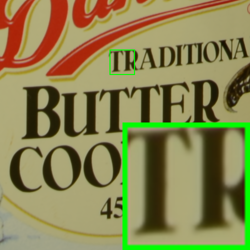
\includegraphics[width=1\textwidth]{images/resize_br_Mean_CC_Noisy_Nikon_D600_ISO_3200_C1_96.png}}
{\footnotesize (e) Mean Image \cite{crosschannel2016}}
\end{minipage}
}
\vspace{-2mm}
\caption{Denoised images of a region cropped from the real noisy image ``Nikon D600 ISO 3200 C1" \cite{crosschannel2016} by different methods. The 
\vspace{-0.5mm}
images are better to be zoomed in on screen.}
\vspace{-2mm}
\label{fig4}
\end{figure*}
\begin{figure*}\vspace{-1mm}
\centering
\subfigure{
\begin{minipage}[t]{0.195\textwidth}
\centering  
\raisebox{-0.15cm}{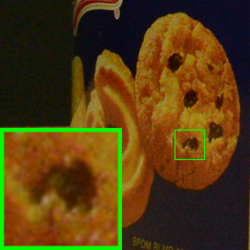
\includegraphics[width=1\textwidth]{images/resize_br_Noisy_CC_Noisy_Nikon_D600_ISO_3200_C1_94b.png}}
{\footnotesize (a) Noisy \cite{crosschannel2016}: 33.77dB  }
\end{minipage}
\begin{minipage}[t]{0.195\textwidth} 
\centering
\raisebox{-0.15cm}{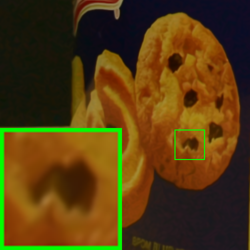
\includegraphics[width=1\textwidth]{images/resize_br_Offline_CC_Noisy_Nikon_D600_ISO_3200_C1_94b.png}}
{\footnotesize (b) External: 36.97dB }
\end{minipage}
\begin{minipage}[t]{0.195\textwidth}
\centering
\raisebox{-0.15cm}{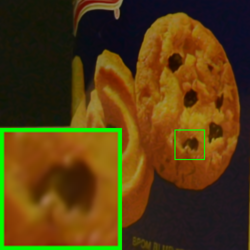
\includegraphics[width=1\textwidth]{images/resize_br_Online_CC_Noisy_Nikon_D600_ISO_3200_C1_94b.png}}
{\footnotesize (c) Internal: 37.40dB }
\end{minipage} 
\begin{minipage}[t]{0.195\textwidth}
\centering
\raisebox{-0.15cm}{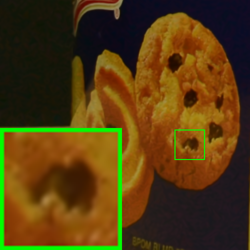
\includegraphics[width=1\textwidth]{images/resize_br_Guided_CC_Noisy_Nikon_D600_ISO_3200_C1_94b.png}}
{\footnotesize (d) Guided Internal: \textbf{38.01}dB }
\end{minipage}
\begin{minipage}[t]{0.195\textwidth}
\centering
\raisebox{-0.15cm}{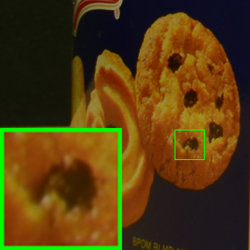
\includegraphics[width=1\textwidth]{images/resize_br_Mean_CC_Noisy_Nikon_D600_ISO_3200_C1_94b.png}}
{\footnotesize (e) Mean Image \cite{crosschannel2016}}
\end{minipage}
}
\vspace{-2mm}  
\caption{Denoised images of a region cropped from the real noisy image ``Nikon D600 ISO 3200 C1" \cite{crosschannel2016} by different methods. The 
\vspace{-0.5mm}
images are better to be zoomed in on screen.}
\vspace{-3mm}
\label{fig5}
\end{figure*}


\subsection{Comparison among external, internal and guided internal priors}

To demonstrate the advantages of external prior guided internal prior learning, in this section we perform real noisy image denoising by methods using external priors (denoted by ``External"), internal priors (denoted by ``Internal"), and the proposed guided internal priors (denoted by ``Guided Internal"), respectively.\ For the ``External" method, we utilize the full external dictionaries (i.e., $r=108$ in Eq.\ (\ref{equ4})) for denoising.\ For the ``Internal" method, the overall framework is similar to the method of \cite{ncsr}.\ A GMM model (with $K = 32$ Gaussians) is directly learned from the PGs extracted from the given noisy image without using any external data, and then the internal orthogonal dictionaries are obtained via Eq.\ (\ref{equ2}) to perform denoising.\ All parameters of the ``External" and ``Internal" methods are tuned to achieve their corresponding best performance. 

We compare the three methods mentioned above on the 60 cropped images from \cite{crosschannel2016}.\ The average PSNR and run time are listed in Table \ref{tab1}.\ The best results are highlighted in bold.\ It can be seen that ``Guided Internal" method achieves better PSNR than both ``External" and ``Internal" methods. In addition, the ``Internal" method is very slow because it involves online GMM learning, while the ``Guided Internal" method is only a little slower than the ``External" method.\ Fig.\ \ref{fig4} and Fig.\ \ref{fig5} show the denoised images of two noisy images by the three methods.\ We can see that the  ``External" method is good at recovering large-scale structures (see Fig.\ \ref{fig4}) while the ``Internal" method is good at recovering fine-scale textures (see Fig.\ \ref{fig5}).\ By utilizing external priors to guide the internal prior learning, our proposed method can effectively recover both the large-scale structures and fine-scale textures. 

\begin{figure*}
\centering
\subfigure{
\begin{minipage}[t]{0.244\textwidth}
\centering
\raisebox{-0.15cm}{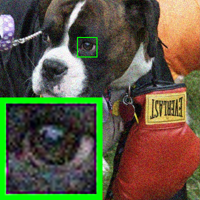
\includegraphics[width=1\textwidth]{images/resize_br_Noisy_dog.png}}
{\footnotesize (a) Noisy \cite{ncwebsite}   }
\end{minipage}
\begin{minipage}[t]{0.244\textwidth}
\centering
\raisebox{-0.15cm}{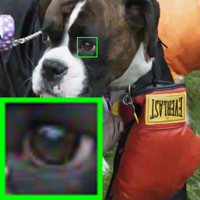
\includegraphics[width=1\textwidth]{images/resize_br_BM3D_dog.png}}
{\footnotesize (b) CBM3D \cite{bm3d,cbm3d}  }
\end{minipage}
\begin{minipage}[t]{0.244\textwidth}
\centering
\raisebox{-0.15cm}{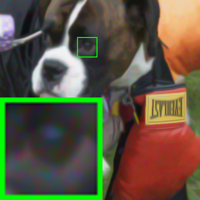
\includegraphics[width=1\textwidth]{images/resize_br_WNNM_dog.png}}
{\footnotesize (c) WNNM \cite{wnnm}   }
\end{minipage}
\begin{minipage}[t]{0.244\textwidth}
\centering
\raisebox{-0.15cm}{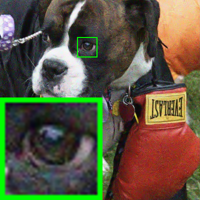
\includegraphics[width=1\textwidth]{images/resize_br_MLP_dog.png}}
{\footnotesize (d) MLP \cite{mlp}  }
\end{minipage}
}\vspace{-3mm}
\subfigure{
\begin{minipage}[t]{0.244\textwidth}
\centering
\raisebox{-0.15cm}{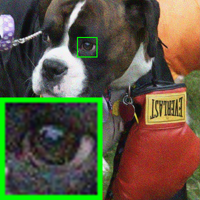
\includegraphics[width=1\textwidth]{images/resize_br_TRD_dog.png}}
{\footnotesize (e) TNRD \cite{chen2015learning}}
\end{minipage}
\begin{minipage}[t]{0.244\textwidth}
\centering
\raisebox{-0.15cm}{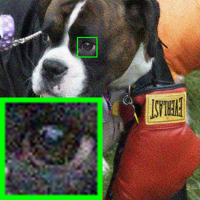
\includegraphics[width=1\textwidth]{images/resize_br_NI_dog.png}}
{\footnotesize (f) NI \cite{neatimage}  }
\end{minipage}
\begin{minipage}[t]{0.244\textwidth}
\centering
\raisebox{-0.15cm}{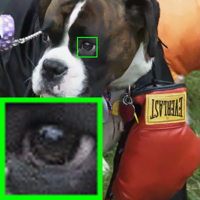
\includegraphics[width=1\textwidth]{images/resize_br_NC_dog.png}}
{\footnotesize (g) NC \cite{noiseclinic,ncwebsite}   }
\end{minipage}
\begin{minipage}[t]{0.244\textwidth}
\centering
\raisebox{-0.15cm}{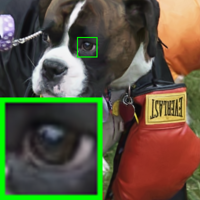
\includegraphics[width=1\textwidth]{images/resize_br_Guided_dog.png}}
{\footnotesize (h) Ours  }
\end{minipage}
}
\vspace{-3mm}
\caption{Denoised images of the real noisy image ``Dog" \cite{ncwebsite} by different methods. The images are better to be zoomed in on screen.}
%\vspace{-1mm}
\label{fig6}
\end{figure*}


\subsection{Comparison with State-of-the-Art Denoising Methods}


We compare the proposed method with state-of-the-art image denoising methods, including CBM3D \cite{bm3d,cbm3d}, WNNM \cite{wnnm}, MLP \cite{mlp}, CSF \cite{csf}, TNRD \cite{chen2015learning}, Noise Clinic (NC) \cite{noiseclinic,ncwebsite}, Neat Image (NI) \cite{neatimage}, and Cross-Channel (CC) \cite{crosschannel2016}.\ Among them, CBM3D, WNNM, MLP, CSF and TNRD are designed based on Gaussian noise model, and they need to know the noise level for denoising.\ We use the method in \cite{noiselevel} to estimate the noise level for them.\ All the other parameters in these methods are set as the default ones.\ Since WNNM, MLP, CSF and TNRD are designed for grayscale images, we use them to denoise the R, G, B channels separately for color noisy images. 

Like our method, the NC is a blind image denoising method which does not need any noise prior.\ The NI is a commercial software for image denoising, which has been embedded into Photoshop and Corel PaintShop \cite{neatimage}.\ The code of CC is not released but its results on the 15 cropped images are available at \cite{crosschannel2016}. Therefore, we only compare with it on the 15 cropped images from \cite{crosschannel2016}. 

\begin{table}
\caption{Average PSNR (dB) and Run Time (seconds) of the ``External", ``Internal", and ``Guided Internal" methods on 60 real noisy images (of size $500\times500\times3$) cropped from \cite{crosschannel2016}.}
\label{tab1}
%\begin{small}
\vspace{-3mm}
\begin{center}
\renewcommand\arraystretch{1}
\begin{tabular}{|c||c|c|c|c|}
\hline
 & \small\textbf{Noisy} &\small \textbf{External} & \small\textbf{Internal} & \small\textbf{Guided Internal}  
\\
\hline
PSNR & 34.51 & 38.21 & 38.07 & \textbf{38.75} 
\\
\hline
Time & | &  \textbf{39.57}  & 587.36 & 41.89
\\
\hline
\end{tabular}
\end{center}\vspace{-2mm}
%\end{small}
\end{table}

\subsubsection{Results on Dataset \cite{ncwebsite}}

Since there is no ``ground truth" for the real noisy images in  dataset \cite{ncwebsite}, we only compare the visual quality of the denoised images by different methods. (Note that method CC \cite{crosschannel2016} is not compared since its code is not available.) Fig.\ \ref{fig6} shows the denoised images of ``Dog". It can be seen that CBM3D and WNNM tend to over-smooth much the image while remaining some noise caused color artifacts.\ MLP and TNRD are likely to remain many noise-caused color artifacts across the whole image. These results demonstrate that the methods designed with Gaussian noise model are not effective for real noise removal.\ Though NC and NI methods are specifically developed for real noisy images, their performance on noise removal is not very satisfactory. In comparison, our proposed method recovers much better the structures and textures (such as the eye area) than the other competing methods. More visual comparisons on this dataset \cite{ncwebsite} can be found in the supplementary file.

\begin{table*}\vspace{2mm}
\caption{PSNR(dB) results of different methods on 15 cropped real noisy images used in \cite{crosschannel2016}.}
\label{tab2}
\begin{center}
\renewcommand\arraystretch{1}
\begin{tabular}{|c||c|c|c|c|c|c|c|c|c|c|}
\hline
Camera Settings & \textbf{Noisy} &\textbf{CBM3D}&\textbf{WNNM}&\textbf{MLP}&\textbf{CSF}&\textbf{TNRD}& \textbf{NI}& \textbf{NC}& \textbf{CC} &\textbf{Ours} 
\\
\hline
\multirow{3}{*}{\small{Canon 5D Mark III}} 
& 37.00 & 37.08 & 37.09 & 33.92 & 35.68 & 36.20 & 37.68 & {\color{blue}{38.76}} & 38.37 & {\color{red}{40.50}}
\\ 
\cdashline{2-11} 
\multirow{3}{*}{ISO = 3200}   
& 33.88 & 33.94 & 33.93 & 33.24 & 34.03 & 34.35 & 34.87 & {\color{blue}{35.69}} & 35.37 & {\color{red}{37.05}}
\\ 
\cdashline{2-11}    
& 33.83 & 33.88 & 33.90 & 32.37 & 32.63 & 33.10 & 34.77 & {\color{blue}{35.54}} & 34.91 & {\color{red}{36.11}}  
\\
\hline
\multirow{3}{*}{Nikon D600} 
& 33.28 & 33.33 & 33.34 & 31.93 & 31.78 & 32.28 & 34.12 & {\color{red}{35.57}} & {\color{blue}{34.98}} & 34.88
\\ 
\cdashline{2-11} 
\multirow{3}{*}{ISO = 3200}   
& 33.77 & 33.85 & 33.79 & 34.15 & 35.16 & 35.34 & 35.36 & {\color{red}{36.70}} & 35.95 & {\color{blue}{36.31}}
\\ 
\cdashline{2-11}    
& 34.93 & 35.02 & 34.95 & 37.89 & 39.98 & {\color{blue}{40.51}} & 38.68 & 39.28 & {\color{red}{41.15}} & 39.23
\\
\hline
\multirow{3}{*}{Nikon D800} 
& 35.47 & 35.54 & 35.57 & 33.77 & 34.84 & 35.09 & 37.34 & {\color{blue}{38.01}} & 37.99 & {\color{red}{38.40}}
\\ 
\cdashline{2-11} 
\multirow{3}{*}{ISO = 1600}   
& 35.71 & 35.79 & 35.77 & 35.89 & 38.42 & 38.65 & 38.57 & 39.05 & {\color{blue}{40.36}} & {\color{red}{40.92}}
\\ 
\cdashline{2-11}    
& 34.81 & 34.92 & 34.95 & 34.25 & 35.79 & 35.85 & 37.87 & 38.20 & {\color{blue}{38.30}} & {\color{red}{38.97}}
\\
\hline
\multirow{3}{*}{Nikon D800} 
& 33.26 & 33.34 & 33.31 & 37.42 & 38.36 & 38.56 & 36.95 & 38.07 & {\color{red}{39.01}} & {\color{blue}{38.66}}
\\ 
\cdashline{2-11} 
\multirow{3}{*}{ISO = 3200}   
& 32.89 & 32.95 & 32.96 & 34.88 & 35.53 & 35.76 & 35.09 & 35.72 & {\color{blue}{36.75}} & {\color{red}{37.07}}
\\ 
\cdashline{2-11}    
& 32.91 & 32.98 & 32.96 & 38.54 & {\color{blue}{40.05}} & {\color{red}{40.59}} & 36.91 & 36.76 & 39.06 & 38.52
\\ 
\hline
\multirow{3}{*}{Nikon D800} 
& 29.63 & 29.66 & 29.71 & 33.59 & 34.08 & {\color{blue}{34.25}} & 31.28 & 33.49 & {\color{red}{34.61}} & 33.76
\\ 
\cdashline{2-11} 
\multirow{3}{*}{ISO = 6400}   
& 29.97 & 30.01 & 29.98 & 31.55 & 32.13 & 32.38 & 31.38 & 32.79 & {\color{blue}{33.21}} & {\color{red}{33.43}}
\\ 
\cdashline{2-11}    
& 29.87 & 29.90 & 29.95 & 31.42 & 31.52 & 31.76 & 31.40 & 32.86 & {\color{blue}{33.22}} & {\color{red}{33.58}}
\\
\hline
Average & 33.41 & 33.48 & 33.48 & 34.32 & 35.33 & 35.65 & 35.49 & 36.43 & {\color{blue}{36.88}} & {\color{red}{ 37.16}}
\\
\hline
%Average SSIM & 0.8483 & 0.8511 & 0.8512 & 0.9113 & 0.9250 & 0.9280 & 0.9126 & 0.9364 & {\color{blue}{0.9481}} & {\color{red}{ 0.9505}}
%\\
%\hline
\end{tabular}
\end{center}
\vspace{1mm}
\end{table*}

\subsubsection{Results on Dataset \cite{crosschannel2016}}

As described in section 4.2, there is a mean image for each of the 17 scenes used in dataset \cite{crosschannel2016}, and those mean images can be roughly taken as ``ground truth" images for quantitative evaluation of denoising algorithms. We firstly perform quantitative comparison on the 15 cropped images used in \cite{crosschannel2016}. The PSNR results of CBM3D \cite{bm3d}, WNNM \cite{wnnm}, MLP \cite{mlp}, CSF \cite{csf}, TNRD \cite{chen2015learning}, NC \cite{noiseclinic,ncwebsite}, NI \cite{neatimage} and
CC \cite{crosschannel2016} are listed in Table \ref{tab2} (The results of CC are copied from the original paper \cite{crosschannel2016}).\ The best and second best PSNR results of each image are highlighted in red and blue, respectively.\ One can see that on 9 out of the 15 images, our method achieves the best PSNR values.\ CC achieves the best PSNR on 3 of the 15 images.\ It should be noted that in the CC method, a specific model is trained for each camera and camera setting, while our method uses the same model for all images.\ On average, our proposed method has 0.28dB PSNR improvements over \cite{crosschannel2016} and much higher PSNR gains over other competing methods.\ Fig.\ \ref{fig7} shows the denoised images of a scene captured by Canon 5D Mark 3 at ISO = 3200.\ We can see that CBM3D, WNNM, NC, NI and CC would either remain noise or generate artifacts, while MLP, TNRD over-smooth much the image.\ By using the external prior guided internal priors, our proposed method preserves edges and textures better than other methods, leading to visually pleasant outputs.\ More visual comparisons can be found in the supplementary file.

We then perform denoising experiments on the 60 images we cropped from \cite{crosschannel2016}.\ The average PSNR results are listed in Table \ref{tab3} (CC is not compared since the code of \cite{crosschannel2016} is not available).\ The best result is highlighted in bold.\ Again, our proposed method achieves much better PSNR results than the other methods.\ The improvement of our method over the second best method (TNRD) is about 1dB. Due to the space limitations, the visual comparisons are provided in the supplementary file.

\begin{table}
\caption{Average PSNR(dB) results of different methods on 60 real noisy images cropped from \cite{crosschannel2016}.}
\vspace{-3mm}
\label{tab3}
\begin{center}
\renewcommand\arraystretch{1}
\begin{tabular}{|c||c|c|c|c|}
\hline
 Methods& \textbf{CBM3D}&\textbf{WNNM}&\textbf{MLP}&\textbf{CSF}
\\
\hline
PSNR &   34.58 & 34.52 & 36.19 & 37.40
\\
\hline
Methods& \textbf{TNRD} & \textbf{NI} & \textbf{NC} &\textbf{Ours} 
\\
\hline
PSNR & 37.75  & 36.53 & 37.57 & {\textbf{{ 38.75}}}
\\
\hline
\end{tabular}
\end{center}\vspace{-4mm}
\end{table}

\begin{figure*}\vspace{1mm}
\centering
\subfigure{
\begin{minipage}[t]{0.195\textwidth}
\centering
\raisebox{-0.15cm}{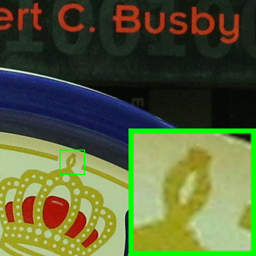
\includegraphics[width=1\textwidth]{images/resize_br_Noisy_5dmark3_iso3200_1_real.png}}
{\footnotesize (a) Noisy  \cite{crosschannel2016}: 37.00dB }
\end{minipage}
\begin{minipage}[t]{0.195\textwidth}
\centering
\raisebox{-0.15cm}{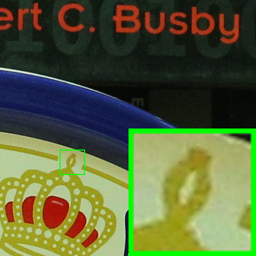
\includegraphics[width=1\textwidth]{images/resize_br_CBM3D_5dmark3_iso3200_1_real.png}}
{\footnotesize (b) CBM3D \cite{bm3d,cbm3d}: 37.02dB}
\end{minipage}
\begin{minipage}[t]{0.195\textwidth}
\centering
\raisebox{-0.15cm}{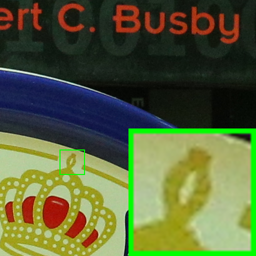
\includegraphics[width=1\textwidth]{images/resize_br_WNNM_5dmark3_iso3200_1_real.png}}
{\footnotesize (c) WNNM \cite{wnnm}: 37.01dB}
\end{minipage}
\begin{minipage}[t]{0.195\textwidth}
\centering
\raisebox{-0.15cm}{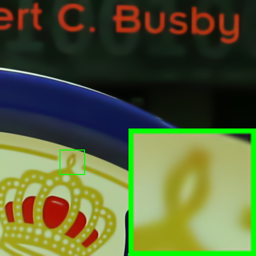
\includegraphics[width=1\textwidth]{images/resize_br_MLP_5dmark3_iso3200_1_real.png}}
{\footnotesize (d) MLP \cite{mlp}: 33.90dB }
\end{minipage}
\centering
\begin{minipage}[t]{0.195\textwidth}
\raisebox{-0.15cm}{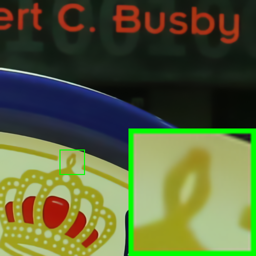
\includegraphics[width=1\textwidth]{images/resize_br_TRD_5dmark3_iso3200_1_real.png}}
{\footnotesize (e) TNRD \cite{chen2015learning}: 36.18dB  } 
\end{minipage}
}\vspace{-3mm}
\subfigure{
\begin{minipage}[t]{0.195\textwidth}
\centering
\raisebox{-0.15cm}{\includegraphics[width=1\textwidth]{images/resize_br_NI_5dmark3_iso3200_1_real.png}}
{\footnotesize (f) NI \cite{neatimage}: 37.68dB  }
\end{minipage}
\begin{minipage}[t]{0.195\textwidth}
\centering
\raisebox{-0.15cm}{\includegraphics[width=1\textwidth]{images/resize_br_NC_5dmark3_iso3200_1_real.png}}
{\footnotesize (g) NC \cite{noiseclinic,ncwebsite}: 38.76dB  }
\end{minipage}
\begin{minipage}[t]{0.195\textwidth}
\centering
\raisebox{-0.15cm}{\includegraphics[width=1\textwidth]{images/resize_br_CCNoise_5dmark3_iso3200_1.png}}
{\footnotesize (h) CC \cite{crosschannel2016}: 38.37dB }
\end{minipage}
\begin{minipage}[t]{0.195\textwidth}
\centering
\raisebox{-0.15cm}{\includegraphics[width=1\textwidth]{images/resize_br_Guided_5dmark3_iso3200_1_real.png}}
{\footnotesize (i) Ours: \textbf{40.50}dB}
\end{minipage}
\begin{minipage}[t]{0.195\textwidth}
\centering
\raisebox{-0.15cm}{\includegraphics[width=1\textwidth]{images/resize_br_Mean_5dmark3_iso3200_1_real.png}}
{\footnotesize (j) Mean Image \cite{crosschannel2016}}
\end{minipage}
}\vspace{-1mm}
\caption{Denoised images of a region cropped from the real noisy image ``Canon 5D Mark 3 ISO 3200 1" \cite{crosschannel2016} by different methods. The images are better to be zoomed in on screen.}
\label{fig7}
\vspace{1mm}
\end{figure*}


\section{Conclusion}

The noise in real-world noisy images is much more complex than additive white Gaussian noise and hard to be modeled by simple analytical distributions such as Gaussian or mixture of Gaussians, making the real noisy image denoising problem very challenging.\ In this paper, we proposed a simple yet effective solution for real noisy image denoising without explicitly assuming certain noise models.\ Specifically, we firstly learned image priors from external clean images, and then employed the learned external priors to guide the learning of internal priors from the given noisy image.\ The learned hybrid priors are utilized for real noisy image denoising.\ Experiments on two real noisy image datasets, where the images were captured under indoor or outdoor lighting conditions by different types of cameras and camera settings, demonstrated that our proposed method achieved much better performance than state-of-the-art image denoising methods.



{
\small
\bibliographystyle{unsrt}
\bibliography{egbib}
}

\end{document}
